% Portable review-manuscript assembly, not publisher camera-ready template.
% Compile from this directory:
% pdflatex main_v10 && bibtex main_v10 && pdflatex main_v10 && pdflatex main_v10
% Portable review build with bibliography, evidence tables, and participant-effect figure.
\documentclass[11pt,a4paper]{article}
\usepackage[margin=1in]{geometry}
\usepackage[T1]{fontenc}
\usepackage{amsmath,amssymb}
\usepackage{booktabs}
\usepackage{graphicx}
\usepackage{tikz}
\usepackage[hidelinks]{hyperref}
\title{Regularisation Validity in Cross-Subject EEG:\\
Prospective Objective Mismatch, Validity Frontiers, and Representation Dependence}
\author{Author and affiliation information pending verification}
\date{}
\begin{document}
\maketitle
\begin{abstract}
Covariance regularisation is usually selected for estimation fidelity,
whereas zero-target cross-subject EEG is evaluated by discrimination on
unseen participants. We examine their mismatch along the complete scalar path
range, sampled using a predeclared finite grid in covariance/tangent-space linear discriminants. An operator
derivation shows that the standardized margin changes through
discriminant-path rotation while covariance predictive loss contains no
class-contrast term. Model selection and representation fitting used
neither target labels nor distribution statistics. On a prospectively
frozen EEGMMIDB block (\(N=20\)), source participant-macro-AUC selection
improved target macro AUC over source covariance-NLL selection by 0.0561
and Ledoit--Wolf by 0.0920 (both Holm-adjusted \(p\) values below 0.006).
The benefit is not uniform: 5/20 and 4/20 participants, respectively,
lost more than 0.02 AUC. In two independently frozen external cohorts
(BNCI2014\_002, \(N=14\); BNCI2015\_001, \(N=12\)), source objective
optima differed in 26/26 outer folds. Target effects were positive
(+0.0176 and +0.0433 versus covariance-NLL) but individually
non-significant after Holm correction (\(p=0.1397\) and 0.1856).
Their validity frontiers spanned 0.0384 and 0.0501 AUC with
cohort-dependent covariance-fidelity budgets. A separate prospective
experiment detected a regularisation-by-representation interaction
(-0.0778 AUC; Holm \(p=0.0133\)), opposite the historical filter-bank
hypothesis. We do not propose a universally superior estimator.
Instead, objective choice emerges as a consequential validity variable
in the studied cross-subject EEG pipelines.
\end{abstract}

\noindent\textbf{Keywords:} EEG; cross-subject decoding; covariance shrinkage;
regularised discriminant analysis; domain generalisation; selection bias;
representation validity.
# SNAPSHOT_SOURCE: lindicaphxag-tech/cs@0b26a5b0853e3b136a92c17e614a3a1936673621 path=papers/eeg-default-regularisation/paper_vnext/01_intro.tex
\section{Introduction}

Cross-subject EEG decoding asks a model trained on one group of participants
to operate on a new person who contributes no labelled calibration trials.
This setting makes regularisation scientifically consequential rather than
merely numerical. Covariance and tangent-space representations can contain
hundreds or thousands of coordinates, while the number of independent source
participants is modest and inter-participant covariance structure is
heterogeneous. Analytic shrinkage therefore provides an attractive default
\cite{ledoit2004,chen2010oas},
but the statistical objective used to stabilise a covariance matrix is not the
same quantity on which a transferred decoder is evaluated.

For a two-class linear discriminant, let
\[
 A_\lambda=(1-\lambda)S+\lambda\nu I,
 \qquad
 w_\lambda=A_\lambda^{-1}d_s,
\]
where \(S\) and \(d_s\) are source within-class covariance and class
contrast. Covariance-fidelity criteria choose \(\lambda\) according to how
well \(A_\lambda\) predicts covariance structure. A held-participant decoder
instead depends on how the inverse-spectrum weighting in \(w_\lambda\)
aligns with that participant's class contrast. These objectives may coincide,
but established covariance-based EEG decoding, including Riemannian
classifiers and filter-bank spatial patterns \cite{barachant2012,ang2012fbcsp},
already provides a framework in which classification risk and covariance
estimation are distinct targets. Our
question is therefore narrower and empirical: \emph{does this distinction
produce a reproducible validity problem in cross-subject EEG when target
information is unavailable?}

Recent EEG research has explored additional model regularisers,
optimal-transport adaptation, cyclic representation transfer and adaptive
spatial--temporal attention
\cite{miao2025freezing,morvay2026wbt,he2026cyclic,ren2026asta}.
Riemannian spatial filtering has also been evaluated with ten decoding
algorithms on six public MI datasets \cite{pan2025rsf}. These studies
establish a high empirical bar, but their primary questions and target
information budgets differ. In particular, unsupervised target-domain
adaptation cannot be ranked against strict zero-target-information (Z0)
selection as though they used identical participant information. Our
primary contribution is thus a mechanism and measurement-validity analysis
inside the predeclared Z0 covariance/tangent-linear-discriminant family,
not a claim to outperform modern domain-adaptive encoders.

The operator geometry makes the distinction precise. For an evaluation
participant with covariance \(\Sigma_g\) and contrast \(d_g\), define the
standardized margin
\[
 m_g(\lambda)=
 \frac{w_\lambda^\top d_g}
 {\sqrt{w_\lambda^\top\Sigma_gw_\lambda}}.
\]
The regularisation-path derivative \(w_\lambda'\) can be decomposed into a
component that only rescales \(w_\lambda\) and a
\(\Sigma_g\)-orthogonal rotation \(r_g\). The scale component cancels from
the standardized margin, giving
\[
 m_g'(\lambda)=
 \frac{r_g(\lambda)^\top d_g}
 {\sqrt{w_\lambda^\top\Sigma_gw_\lambda}}.
\]
In contrast, the covariance-predictive NLL derivative contains covariance
operators but no class-contrast vector. Hence a covariance optimum is not, in
general, a discriminative stationary point. Around an interior covariance
optimum, covariance regret is second order in path displacement whereas a
non-zero margin derivative is first order. This supplies a mechanistic reason
why a shallow covariance-fidelity basin can admit materially different
decisions without claiming that such fragility must occur in every EEG cohort.

The historical version of this study could not establish that chain. Its
regularisation grid excluded the near-zero analytic-shrinkage region; a
proposed transfer proxy squared a cross-participant margin and therefore lost
direction information; several summary-table gains could not be traced to one
machine-readable configuration lineage; and an apparent filter-bank advantage
mixed representation and regularisation effects. We therefore reconstruct the
study from participant-level artifacts, full-domain paths and explicitly
frozen evidence tiers. Historical rows with unresolved arithmetic or
provenance are quarantined rather than repaired by inference.

The first prospective test, EEGMMIDB S021--S040, was frozen before any target
outcome and used a strict Z0 information budget: no target labels, target
feature moments, target-fitted geometry or target distribution statistics
entered representation or regularisation selection. It tests whether the
source objective separation has a held-participant consequence. Negative
algorithm results are retained with equal status: lower-tail signed selection
failed to improve over correctly nested source tuning, and a
covariance-fidelity-constrained selector was prospectively inferior on a
separate EEGMMIDB block. These failures prevent the paper from turning a
measurement-validity finding into an unsupported new-estimator story.

We next recover a stronger external evidence tier. BNCI2014\_002 and
BNCI2015\_001 were frozen under one TRUE PRE-DATA protocol before project
access to their outcomes. Each cohort uses its native montage, full outer
leave-one-participant-out evaluation, participant-grouped inner selection and a
dense regularisation path whose target scores are frozen before AUC
calculation. These datasets test both source-objective separation and a
post-S021 Regularisation Validity Frontier. The frontier does not ask for a
target-optimal \(\lambda\); it asks how much held-participant AUC variation
is compatible with a specified amount of source covariance-fidelity regret.
A pre-outcome mathematical correction replaces a structurally meaningless
generic zero-crossing statistic with material-fragility budgets for 0.01,
0.02 and 0.05 AUC envelope spans.

A separate prospectively frozen EEGMMIDB S041--S060 experiment asks a
different scientific question: can regularisation objective change the
conclusion drawn about EEG representations? It compares a wide-band
231-dimensional tangent representation, an eight-band 1848-dimensional
filter-bank representation, a source-only matched-dimension filter-bank PCA
control and a label-independent nuisance-dimension control. This design
permits the original hidden-filter-bank hypothesis to fail. A source-budget
intervention further tests whether a simple monotonic feature-to-sample ratio
law is sufficient to explain any objective mismatch.

Accordingly, the contribution is an evidence chain rather than a leaderboard.
We (i) derive the path-rotation condition that separates covariance fidelity
from discriminative transfer; (ii) test the complete scalar domain under
participant-grouped source selection; (iii) prospectively evaluate the target
consequence and its harmed-participant tail; (iv) replicate source-objective
separation in two TRUE PRE-DATA external cohorts while preserving
dataset-level inferential boundaries; (v) quantify corrected, uncertainty-aware
regularisation validity frontiers; and (vi) prospectively test whether the
choice of regularisation objective changes a representation conclusion. We do
not claim a universal EEG regularisation law, a universal multiplier, or a
state-of-the-art replacement covariance estimator.

\section{Methods}

\subsection{Evidence tiers and target-information budgets}
Every analysis is assigned an evidence role before interpretation.
Development or post-hoc analyses may use already exposed cohorts but cannot
prospectively confirm a later method or claim. A prospective block is frozen
before target outcomes are opened. TRUE PRE-DATA external replication further
requires that the scientific protocol predates project access to that
dataset's outcomes.

Target information is tracked separately. Z0 uses no target labels, target
feature moments, target batch-normalisation statistics, target quality
thresholds or target-fitted geometry for model selection before scores are
frozen. U-\(k\) permits a predeclared first \(k\) unlabeled target trials
for an unsupervised calibration statistic. U-all permits the complete
unlabeled target batch and is explicitly transductive. Headline
regularisation claims use Z0.

\subsection{EEG cohorts and representations}
The PhysioNet EEGMMIDB protocol uses runs R04, R08 and R12, a fixed set of 21
FC/C/CP sensorimotor channels and every recorded T1/T2 cue epoch from
0.5--3.5~s. BAD annotations are retained as quality flags rather than
silently deleting task cues. Trial covariances use divisor \(T\), a
trace-proportional numerical SPD floor and a source-fitted tangent reference.

The primary wide representation uses 8--30~Hz and has 231 tangent
coordinates. The prospective representation experiment additionally uses
eight fixed 4-Hz bands from 8--40~Hz (FB8-1848), a source-only PCA projection
of that filter bank to 231 dimensions (FB8-SOURCE-PCA231), and a
1848-dimensional WIDE+NUISANCE control obtained by appending
label-independent source-scaled nuisance coordinates to WIDE231.

The TRUE PRE-DATA v5 external cohorts use their complete frozen native
montages rather than a performance-selected common montage.
BNCI2014\_002 contains 14 participants, 15 EEG channels and 120 tangent
coordinates. BNCI2015\_001 contains 12 participants, 13 EEG channels and
91 tangent coordinates, with every session returned by the pinned dataset
loader retained. Both use their official 5-s motor-imagery task interval,
8--30~Hz filtering, resampling to 160~Hz and a source-only tangent reference.

\subsection{Scalar regularisation path and source objectives}
For identity shrinkage,
\[
 A_\lambda=(1-\lambda)S+\lambda\nu I,
 \qquad
 \nu=\operatorname{tr}(S)/p,
\]
the frozen primary selection grid is
\[
\begin{aligned}
\Lambda=\{&
0,.0005,.001,.002,.003,.005,.0075,.01,.015,.02,.03,.05,.075,\\
&.10,.15,.20,.30,.40,.50,.60,.70,.80,.90,.95,.98,.99,1
\}.
\end{aligned}
\]
Candidates that are singular at machine precision are marked infeasible
rather than silently altered. The phrase 'full-domain' denotes that the
predeclared finite candidate grid spans the endpoints and near-zero analytic
shrinkage region of [0,1]; it does not assert continuous optimisation or a
proof that no finer-grid optimum exists. A separate 405-point grid supports
post-score frontier discretisation sensitivity.

Inside each participant-grouped source-validation fold, every
representation-dependent operation is refitted without the held source
participant, including tangent geometry and, where applicable, PCA. Two
source objectives are measured on the same held-source participants:
participant-macro AUC, which is maximised, and covariance predictive NLL,
which is minimised. Analytic Ledoit--Wolf and OAS are fitted on the same final
source feature matrix. One-standard-error sets are reported only as
operational sensitivity regions and are not called formal equivalence sets.

\subsection{Operator geometry of objective mismatch}
The source-trained discriminant is
\[
 w_\lambda=A_\lambda^{-1}d_s,
\]
and
\[
 B=\frac{dA_\lambda}{d\lambda}=\nu I-S,
 \qquad
 w_\lambda'=-A_\lambda^{-1}Bw_\lambda.
\]
For an evaluation participant with within-class covariance \(\Sigma_g\)
and class contrast \(d_g\), define the standardized signed margin
\[
 m_g(\lambda)=
 \frac{w_\lambda^\top d_g}
 {\sqrt{w_\lambda^\top\Sigma_gw_\lambda}}.
\]
We decompose path motion into a scale component and a
\(\Sigma_g\)-orthogonal rotation:
\[
 \alpha_g=
 \frac{w_\lambda'^\top\Sigma_gw_\lambda}
 {w_\lambda^\top\Sigma_gw_\lambda},
 \qquad
 r_g=w_\lambda'-\alpha_gw_\lambda.
\]
By construction \(r_g^\top\Sigma_gw_\lambda=0\), and direct
differentiation gives
\[
 m_g'(\lambda)=
 \frac{r_g^\top d_g}
 {\sqrt{w_\lambda^\top\Sigma_gw_\lambda}}.
\]
Thus pure rescaling of a discriminant cannot alter its standardized margin;
only path rotation aligned with the evaluation contrast can do so.

For covariance predictive NLL per dimension,
\[
 C_g(\lambda)=\frac{1}{p}
 \left[
 \log\det A_\lambda+
 \operatorname{tr}(A_\lambda^{-1}\Sigma_g)
 \right],
\]
the derivative is
\[
 C_g'(\lambda)=\frac{1}{p}
 \left[
 \operatorname{tr}(A_\lambda^{-1}B)
 -
 \operatorname{tr}
 (A_\lambda^{-1}BA_\lambda^{-1}\Sigma_g)
 \right],
\]
which contains no class-contrast term. Therefore
\(C_g'(\lambda_C)=0\) does not imply \(m_g'(\lambda_C)=0\).
If an interior covariance optimum has finite positive curvature,
Taylor expansion gives covariance regret
\(C_g(\lambda_C+h)-C_g(\lambda_C)=O(h^2)\), whereas a nonzero
margin derivative produces \(m_g(\lambda_C+h)-m_g(\lambda_C)=O(h)\).
The resulting local \(\sqrt{\text{regret}}\) relation is explicitly
conditional on an interior stationary point. It is not invoked as a local
asymptotic explanation for outer folds whose covariance optimum lies at
\(\lambda=0\) or 1; those folds are handled directly by the empirical
finite-path validity envelope. These quantities are analysis-only diagnostics
and never select a target model.

\subsection{EEGMMIDB prospective target test and source-pool sensitivity}
For S021--S040, source participants S001--S008, WIDE231, the complete scalar
path and two paired target comparisons were frozen before any target outcome.
The primary contrasts are source-macro selection versus Ledoit--Wolf and
source-macro selection versus source covariance-NLL selection. Target labels
enter only after source fitting and target score generation.

Participant resampling does not represent uncertainty in the shared source
pool. A post-primary delete-one-source audit therefore omits each of
S001--S008 in turn, recomputes every inner tangent reference, reruns the
complete regularisation path, reselects both source objectives, rebuilds the
final geometry and refits the classifiers before rescoring the fixed target
block. This sensitivity is not assigned a second confirmatory p-value.

\subsection{TRUE PRE-DATA external v5 protocol}
BNCI2014\_002 and BNCI2015\_001 were frozen under one v5 protocol before
project access to either cohort's outcomes. Outer evaluation is full
leave-one-participant-out. Inner source folds are participant-grouped and
determined without target information. Every outer fold writes and SHA-256
hashes the complete predeclared target score family before target labels are
used for AUC calculation.

Primary methods are Ledoit--Wolf LDA, OAS LDA, source covariance-NLL
full-domain LDA, source participant-macro-AUC full-domain LDA,
tangent-space logistic regression and Riemannian MDM. Two post-S021
secondary selectors were also frozen before these external outcomes.

The discriminability-first lexicographic selector defines
\[
 \mathcal D_\epsilon=
 \{\lambda:A_s(\lambda)\ge A_s^*-\epsilon\},
 \qquad \epsilon=0.01,
\]
and chooses the member of \(\mathcal D_\epsilon\) with minimum source
covariance NLL.

The mean--tail--fidelity selector first retains candidates within 0.01 AUC of
the best source mean, then maximises the CVaR25 of held-source participant
AUC, retains candidates within 0.005 AUC of the best CVaR25, and finally
minimises source covariance NLL. Its predeclared promotion rule requires a
target mean-bootstrap lower bound above -0.01 AUC, no increase in the
>0.02 harm rate and non-negative target paired CVaR25 in at least two
independent external cohorts; otherwise it remains secondary.

\subsection{Corrected Regularisation Validity Frontier}
For outer target participant \(g\), let
\[
 r_g(\lambda)
 =
 C_g^{\mathrm{source}}(\lambda)
 -
 \min_{\lambda'}C_g^{\mathrm{source}}(\lambda')
\]
be the source-only covariance predictive-NLL regret associated with the
source pool that excludes participant \(g\). Let \(A_g(\lambda)\) be the
target AUC obtained from the already frozen dense-path score vector.

At the cohort level,
\[
 \bar r(\lambda)=\frac{1}{G}\sum_g r_g(\lambda),
 \qquad
 \bar A(\lambda)=\frac{1}{G}\sum_g A_g(\lambda).
\]
Because outer folds can have slightly different covariance optima, we use the
finite-grid excess coordinate
\[
 \widetilde r(\lambda)=
 \bar r(\lambda)-\min_{\lambda'}\bar r(\lambda').
\]
For budget \(\delta\),
\[
 \mathcal A_\delta=
 \{\lambda:\widetilde r(\lambda)\le\delta\},
\]
and the AUC validity envelope is
\[
 E_{AUC}(\delta)=
 \left[
 \min_{\lambda\in\mathcal A_\delta}\bar A(\lambda),
 \max_{\lambda\in\mathcal A_\delta}\bar A(\lambda)
 \right].
\]
The maximum envelope span is reported over the dense path. The primary
material-fragility budget is
\[
 \delta_{0.02}
 =
 \inf\{\delta:
 \operatorname{span}(E_{AUC}(\delta))\ge0.02\}.
\]
Thresholds 0.01 and 0.05 are descriptive sensitivity analyses.

This definition replaces a generic centered-AUC zero-crossing statistic that
was identified as structurally uninformative before the first v5 target
outcome: the covariance-optimal path point has zero centered difference by
construction. Zero-crossing budgets are retained only for genuinely signed
external scientific contrasts.

Raw per-dimension NLL regret is primary. Regret divided by held-source NLL SD
or SE at the covariance optimum is reported as scale-aware sensitivity. The
dense path uses 0.0025 spacing plus the frozen near-zero anchors. Strict
subsets with strides 1, 2, 4 and 8 audit grid discretisation.

\subsection{Frontier uncertainty}
The participant is resampled as a paired path. For each of 20,000 bootstrap
draws, one participant-index vector is sampled and reused for every
\(\lambda\); \(\bar r(\lambda)\), \(\bar A(\lambda)\), the finite-grid
regret minimum, the envelope and each \(\delta_\tau\) are then recomputed.
We report a percentile interval for maximum envelope span, the fraction of
draws in which each material threshold is reachable and, conditional on a
finite threshold, its percentile interval. No bootstrap path is used to
select a deployed method.

\subsection{Post-outcome simultaneous-path frontier sensitivity}
After inspecting the external outcomes, we identified a second-order
inference concern: percentile-bootstrap intervals for a data-selected
max--min path span need not account for path-wide extremum selection.
We therefore implement a supplementary simultaneous sensitivity audit on
the archived \(G\times L\) target AUC matrix. For each participant bootstrap
replicate, exactly one index vector is shared across all \(L\) lambda points.
Let \(q_{1-\alpha}\) be the bootstrap quantile of the supremum norm
\(\|\bar A^*-\bar A\|_\infty\). A simultaneous ordinate deviation no
larger than \(q_{1-\alpha}\) implies the span differs from the observed
span by no more than \(2q_{1-\alpha}\). We subtract twice this bound from
every empirical validity-envelope span to define a conservative
post-outcome sensitivity curve and report the first fixed empirical
NLL-regret budget at which its lower curve reaches 0.02 AUC.

This audit uses a paired whole-path resample, not 405 uncorrected
pointwise intervals. It treats the source-regret axis as estimated but
fixed, ignores uncertainty from overlapping outer source models, and
does not cover acquiring new datasets. It is therefore a nominal
conditional sensitivity diagnostic, not a new pre-registered test or a
distribution-free confidence certificate. The complete procedure is
implemented by src/frontier\_simultaneous\_path\_sensitivity.py.

\subsection{V11 translation-invariant real-artifact inference reanalysis}
The initially implemented absolute-ordinate supremum bootstrap incorporates
nuisance variability in the cohort's overall AUC level, despite the fact
that adding one constant to a participant's entire AUC path does not change
its \(\lambda\)-dependent range. We therefore augment the V10 path
sensitivity with the oscillation seminorm
\[
 \operatorname{osc}(e)=\max_\lambda e(\lambda)-\min_\lambda e(\lambda).
\]
For every bootstrap draw, target participants are resampled in groups with
their full 405-point AUC trajectories intact. The empirical error
\(e^*(\lambda)=\bar A^*(\lambda)-\bar A(\lambda)\) is evaluated as a whole
path, and its oscillation is stored. The 95th percentile of this empirical
oscillation distribution defines a nominal, post-outcome, translation-
invariant sensitivity radius \(q_{\mathrm{osc}}\). Since a span functional
is 1-Lipschitz in this seminorm, we examine
\[
 L_{\mathrm{osc}}=\max(0,\operatorname{osc}(\bar A)-q_{\mathrm{osc}}).
\]
Any material-fragility budget corrected by this method holds the estimated
source covariance-regret path fixed. Resampling target participants cannot
quantify refit uncertainty from shared/overlapping outer source sets.
The result is an exploratory conditional sensitivity assessment and not
a formal uniform population confidence interval. The raw external input SHA-256 checksums, workflow artifact IDs, seed,
20,000 resamples and outputs are recorded in the versioned v11 evidence
receipt supplied with the repository.

\subsection{Prospective representation interventions}
The S041--S060 block compares four prespecified representations:
WIDE231, FB8-1848, FB8-\allowbreak SOURCE-\allowbreak PCA231 and
WIDE+\allowbreak NUISANCE1848, under matched target-information budgets. A separate
source-budget intervention retains fixed fractions
\(\{1,.75,.50,.25\}\) within each source participant-by-class cell while
holding the target set, channels, frequency definition and feature
construction fixed. Neither representation nor budget is chosen from target
performance.

\subsection{Calibration-budget identifiability control}
The S061--S080 deployment-budget block compared Z0 with U5/U10/U20-prefix
and U-all variants of a source-frozen linear score. The tested unlabeled
adaptation subtracts a constant target-participant feature translation
\(b_k\):
\[
 s_k(x)=w^\top(x-b_k-c)=s_0(x)-w^\top b_k.
\]
Within one participant, this is a constant score shift and therefore cannot
change ROC ordering or ROC AUC. Consequently, a zero AUC contrast for this
specific calibration operator is an algebraic identifiability result rather
than evidence that unlabeled calibration is generally useless. Any practical
calibration follow-up must use a threshold-sensitive endpoint and is
post-outcome relative to this experiment.

\subsection{Statistical inference and risk reporting}
The participant is the primary inferential unit; trials and sessions are not
treated as independent replicates. Paired contrasts report mean, median, Q25,
Q10, Q05, worst participant, improved count, harm rates below -0.01 and
-0.02, CVaR25, CVaR10 and a 20,000-resample participant bootstrap interval.
Exact sign-flip tests are used for \(N\le20\), and Holm correction is
applied to the predeclared H2/H3 family within each dataset.

Datasets are replication strata. External cohorts are reported separately
before equal-dataset descriptive summaries. Trials are never pooled across
datasets as iid evidence, and leave-one-dataset-out direction analysis is not
treated as informative until at least three eligible datasets exist.
BNCI2015\_001 session-specific results are descriptive within-participant
robustness analyses only.

\subsection{Post-outcome individual-harm and influence sensitivity}
To characterize heterogeneous benefit without selecting an alternative
policy from visible target labels, a supplementary diagnostic takes only
the frozen paired per-participant effect vectors. Material harm is defined
as a paired AUC decrease strictly greater than 0.02 in magnitude. For each
of the six cohort--comparator contrasts, we report the harmed count and
fraction, the median, the symmetric 10\%-trimmed mean, and the full range
of delete-one-target-participant means. A conventional two-sided 95\%
Wilson interval provides a conditional iid-participant reference for the
harm fraction. It is not a simultaneous interval, makes no allowance for
source-fit dependence, and is not a population-of-datasets safety bound.
These calculations were developed after all three cohorts had been
observed and are not added to any frozen primary testing family. A
delete-one-target calculation must not be confused with full
delete-one-source refitting and reselection.

\subsection{Result lineage and fail-closed receipts}
Every admitted confirmatory result records exact participant IDs,
participant/session trial counts, channel list and tangent dimension,
target-information budget, environment, source/target fold membership,
method-set identity, full source criteria by \(\lambda\), workflow commit,
dataset/raw-file identities when available, result JSON hash and score-family
hash. The v5 receipt validator additionally verifies that target scores were
frozen before label-based AUC evaluation. Manuscript tables are rendered from
absolute machine-readable metrics; manually supplied gain columns are
forbidden. Historical rows whose provenance cannot be reconciled remain
excluded rather than silently repaired.

\section{Results}

\subsection{The full source domain separates covariance fidelity from discrimination}
The first reviewer-critical test used authentic EEGMMIDB source data from
S001--S008 (360 original task trials) and expanded the scalar path to the
complete \([0,1]\) domain, including the analytic-shrinkage neighbourhood.
With participant-grouped source validation, the macro-AUC optimum occurred at
\(\lambda=0.8\) (0.67833), whereas held-source covariance predictive NLL was
minimised at \(\lambda=0.075\). Ledoit--Wolf and OAS fitted on the final
source representation selected 0.01567 and 0.01953, respectively. The
low-regularisation region was therefore available rather than excluded by
construction.

The separation is visible over the path rather than only at the selected
values. Source macro AUC rises from 0.55732 at \(\lambda=0.015\) to 0.62032
at 0.075, 0.66251 at 0.5 and 0.67833 at 0.8. Covariance NLL moves in the
opposite direction after its optimum: -2.56323 at 0.075, -1.93560 at 0.5 and
-1.64090 at 0.8. The discriminability and covariance one-standard-error
admissible sets overlap only at 0.075 and 0.10 (Jaccard 0.125). Choosing the
covariance-NLL optimum instead of the discriminability optimum costs 0.05801
source macro-AUC; choosing the discriminability optimum increases covariance
NLL by 0.92233. These are source-only mechanism results and do not establish
an unseen-target gain.

\subsection{Strict Z0 execution is feasible, but two targets do not establish efficacy}
The first official EDF feasibility run held out S009 and S010 while using
S001--S008 as source. All 90 target task cues were retained and no target
data entered geometry or parameter selection. On S009, Ledoit--Wolf,
source-participant nested shrinkage and the source-signed/tail controls
obtained AUC 0.57143, 0.57540 and 0.58135, respectively. On S010,
Ledoit--Wolf obtained 0.79960 while nested shrinkage and the signed/tail
controls obtained 0.77183 and 0.77976. This deliberately small block therefore
demonstrates protocol integrity and target heterogeneity, not efficacy.

\subsection{The BNCI objective separation survives a full-domain stress test}
A first BNCI2014\_001 experiment evaluated all nine participants in outer
LOSO with 288 left/right motor-imagery trials per participant. The initial
development grid began at 0.2; hence its apparent benefit over analytic
shrinkage could not answer the reviewer's search-space objection. After those
target outcomes had been exposed, we therefore ran a disclosed post-hoc
stress audit over the complete \([0,1]\) domain. It is not treated as
independent confirmation.

Across the nine outer folds, analytic Ledoit--Wolf selected
\(\lambda=0.00227\)--0.00355. The source covariance-NLL optimum was 0.10 in
all nine folds, whereas the source participant-macro-AUC optimum was 0.50 in
one fold, 0.90 in two and 0.95 in six. Thus restoring the near-zero region did
not move the discriminability optimum towards analytic shrinkage.
Participant-macro target AUC was 0.75291 for Ledoit--Wolf, 0.75295 for OAS,
0.76475 for logistic regression, 0.77182 for the source covariance-NLL
optimum and 0.78646 for the full-domain source-discriminability optimum.
The latter exceeded Ledoit--Wolf by a descriptive mean 0.03355 AUC (7/9
participants improved; exact sign-flip \(p=0.03125\)). Because the same nine
targets had been exposed previously, this effect is classified as post-hoc
mechanism stress evidence rather than a confirmatory generalisation result.

\subsection{Prospective falsification removes two candidate replacement rules}
The preregistered lower-tail signed selector did not improve over nested
source-participant scalar tuning in the initial BNCI2014\_001 run: its
participant-macro AUC was 0.78455 versus 0.78782 for nested source-macro-AUC
tuning, a mean paired difference of -0.00328, with a worst participant
difference of -0.04070. It is therefore retained as a direction-aware
mechanism control rather than a superior algorithm.

A separate candidate, covariance-fidelity-constrained transfer shrinkage
(CFCTS), was frozen before evaluating EEGMMIDB S011--S020. The source set
remained S001--S008 and the information budget was Z0. Mean AUC was 0.66730
for the preregistered nested comparator and 0.63309 for CFCTS, a paired mean
difference of -0.03421 (participant bootstrap 95\% CI
[-0.05593,-0.01190], exact two-sided sign-flip \(p=0.02734\)). Six of ten
participants were harmed by more than 0.02 AUC and the worst difference was
-0.08893. CFCTS is therefore rejected as the primary correction rather than
retuned on these participants.

\subsection{Prospective full-domain mismatch predicts an untouched 20-participant target block}
The full-domain S021--S040 experiment was frozen before any target outcome.
Source participants remained S001--S008; the target-information budget was
Z0; every original task cue was retained. The source-only path selected
\(\lambda_D=0.8\) for participant discriminability and \(\lambda_C=0.075\)
for covariance predictive NLL, while the final source Ledoit--Wolf and OAS
values were 0.01567 and 0.01953.

Across the 20 untouched target participants, participant-macro AUC was
0.62919 for Ledoit--Wolf, 0.63562 for OAS, 0.67003 for logistic regression,
0.66509 for source covariance-NLL selection and 0.72116 for full-domain
source-discriminability selection. Relative to Ledoit--Wolf, the latter
improved mean participant AUC by 0.09197 (median 0.07133; 16/20 participants
improved; participant-bootstrap 95\% CI [0.04108,0.14310]; exact
\(2^{20}\) sign-flip \(p=0.00255\); Holm-adjusted \(p=0.00510\)).
Relative to the stronger source covariance-NLL comparator, the improvement
was 0.05607 (median 0.05929; 15/20 improved; 95\% CI
[0.02185,0.09049]; exact sign-flip and Holm-adjusted \(p=0.00597\)).

The effect was not universal. Four participants were harmed by more than
0.02 AUC relative to Ledoit--Wolf and five relative to covariance-NLL
selection; the worst paired changes were -0.11067 and -0.07312,
respectively. The prospective result therefore supports a target consequence
of the objective mismatch while motivating a separate hard-participant
reliability analysis.

A stricter post-primary delete-one-source sensitivity propagated source-pool
variation through the entire analysis rather than fixing the original
hyperparameter. After omitting each of S001--S008 in turn, we recomputed every
inner source tangent reference, reran the complete \([0,1]\) path, reselected
both the discriminability and covariance-NLL optima, rebuilt the final tangent
reference and refit the classifiers. The discriminability-selected strength
varied across \(\{0.4,0.8,0.95\}\), whereas the covariance-NLL optimum was
0.075 in seven omissions and 0.10 in one, demonstrating genuine source-pool
selection uncertainty. Nevertheless, discriminability-selected macro AUC was
0.71272 on average across omissions (SD 0.00926; range
0.69999--0.72581). Its advantage over a freshly reselected covariance-NLL
model remained positive in 8/8 omissions (mean +0.05556; range
+0.04329 to +0.07172), and its advantage over a freshly refit Ledoit--Wolf
model was also positive in 8/8 (mean +0.10079; range +0.07069 to +0.13741).
This is a post-primary training-pool sensitivity analysis, not an additional
confirmatory hypothesis test, but it directly shows that the prospective
effect does not depend on one source participant or on freezing the originally
selected lambda.

A separate deterministic score-regeneration audit then rebuilt all five
prospective target methods from the immutable S021--S040 trial-covariance
artifact and the frozen implementation semantics. Across all 20 target
participants and five methods, regenerated AUCs matched the workflow table at
the stored eight-decimal precision (maximum absolute difference 0.0).
This closes a result-lineage gap without rewriting the original chronology:
the original workflow did not archive an independent trial-score file, so the
regenerated score hashes are explicitly post-hoc reproducibility evidence
rather than an original score freeze.

\subsection{Two TRUE PRE-DATA external cohorts replicate source-objective separation and preserve the target-effect direction}
The external v5 panel was frozen before project access to either
BNCI2014\_002 or BNCI2015\_001 outcomes. The scientific runner, source
selection rules, dense path, secondary selectors and score-freeze contract
were fixed before the first cohort was opened. BNCI2015\_001 was then
executed with byte-identical scientific assets; its execution-only child PR
changed only the CI trigger. BNCI2014\_002 contributed 14 participants,
15 native EEG channels and 2240 target trials. BNCI2015\_001 contributed
12 participants, 13 native channels and 5600 target trials across two or
three sessions per participant. Both analyses were Z0.

Source-objective separation was complete across the external panel. In
BNCI2014\_002, source participant-discrimination and covariance-NLL selected
different strengths in 14/14 outer folds: the discrimination optimum lay
between 0.7 and 0.9, while the covariance optimum was zero in 13 folds and
0.02 in one. In BNCI2015\_001 they differed in 12/12 folds: the
discrimination optimum was 0.9 or 0.95, while covariance-NLL selected
0.015--0.05. Thus the two TRUE PRE-DATA cohorts contain 26/26 outer folds
with different source objective optima. This fold count is descriptive
consistency within two datasets, not 26 independent replication strata.

The target consequence had the same direction in both datasets but the
frozen small-sample exact tests remained individually inconclusive. In
BNCI2014\_002, participant-macro AUC was 0.77810 for source-macro selection,
0.76047 for covariance-NLL and 0.75523 for Ledoit--Wolf.
Source-macro minus covariance-NLL was +0.01763 AUC
(95\% participant-bootstrap CI [-0.00358,0.03728], exact sign-flip
\(p=0.12329\), Holm \(p=0.13965\)); source-macro minus Ledoit--Wolf was
+0.02287 (95\% CI [0.00045,0.04402], Holm \(p=0.13965\)).
In BNCI2015\_001, the corresponding AUCs were 0.76697, 0.72368 and 0.72166.
The source-macro advantages were +0.04329 over covariance-NLL
(95\% CI [0.00016,0.09345], exact \(p=0.10107\), Holm
\(p=0.18555\)) and +0.04531 over Ledoit--Wolf
(95\% CI [0.00290,0.09565], exact \(p=0.09277\), Holm
\(p=0.18555\)). The equal-dataset descriptive means of H2 and H3 were
+0.03046 and +0.03409 AUC, respectively. We therefore describe the target
effect as directionally replicated across both TRUE PRE-DATA cohorts, not as
two individually significant superiority confirmations.

The harmed-participant tail persisted. For H2, three of 14 BNCI2014\_002
participants and two of 12 BNCI2015\_001 participants lost more than
0.02 AUC; the corresponding CVaR25 values were negative. The predeclared
mean--tail--fidelity selector therefore remained secondary: its change versus
pure source-macro selection was +0.00416 in BNCI2014\_002 and +0.00055 in
BNCI2015\_001, with negative target CVaR25 in both. A descriptive audit of
the simpler discriminability-first lexicographic selector also failed to
support promotion, with mean changes of -0.00865 and -0.00753 AUC relative
to pure source-macro selection. The external evidence therefore strengthens
the objective-mismatch finding without producing a superior new selector.

BNCI2015\_001 additionally supplied the predeclared descriptive
cross-session check. Source-macro minus covariance-NLL was positive on average
within sessions 0A, 1B and 2C (+0.06252, +0.05296 and +0.06270 AUC,
respectively); source-macro minus Ledoit--Wolf was similarly positive
(+0.06495, +0.05432 and +0.06657). Session rows were not used as independent
inferential units.

\subsection{Post-outcome participant-harm uncertainty and influence}
To check whether positive cohort means conceal negative transfer, we performed
an explicitly post-outcome sensitivity audit of all six frozen participant
effect vectors (three cohorts by two covariance comparators). Relative to
source covariance-NLL, the numbers of participants losing more than 0.02 AUC
were 5/20 in EEGMMIDB S021--S040, 3/14 in BNCI2014\_002 and 2/12 in
BNCI2015\_001; the corresponding Ledoit--Wolf counts were 4/20, 2/14 and
2/12. For the covariance-NLL contrasts, 95\% Wilson iid-participant
reference intervals for those harm fractions were [0.112, 0.469],
[0.076, 0.476] and [0.047, 0.448], respectively. These intervals are
conditional descriptive references, not source-pool or new-dataset safety
guarantees, because the target participants share fitted source models.

The frozen 46-person individual effect distribution is visualised in
Fig.~\ref{fig:participant-harm-v10}; the plot is descriptive rather than
an additional independent experiment.

An additional post-outcome influence calculation removed one target
participant at a time without refitting the shared source model. The smallest
remaining mean effects versus covariance-NLL were +0.0475, +0.0142 and
+0.0258 AUC in the same dataset order. Thus the observed positive
within-cohort mean directions do not depend on any single test participant.
However, BNCI2015\_001 had a mean gain of +0.0433 but a median gain of only
+0.0105, indicating a right-skewed benefit distribution. Neither this
delete-one diagnostic nor its positive direction supplies a new
confirmatory test or resolves the substantial harmed-participant tail.
The exact participant-level audit is reproducible by
src/participant\_harm\_influence\_audit.py using the immutable three-cohort
paired-effect receipt.

\subsection{Corrected TRUE PRE-DATA validity frontiers show reproducible decision variation but cohort-specific steepness}
The original v5 runner emitted a generic zero-crossing statistic for an AUC
path centered on its own covariance optimum. That statistic was identified as
structurally uninformative before the first v5 target result became available:
the covariance-optimal point has zero centered difference by construction and
therefore places zero inside every non-negative admissibility set. Following
the frozen pre-outcome correction, we instead report the complete
covariance-regret--AUC envelope, its maximum span, and the
material-fragility budget
\[
 \delta_\tau=
 \inf\{\delta:
 \operatorname{span}(E_{AUC}(\delta))\ge\tau\},
\]
with \(\tau=0.02\) AUC primary and 0.01/0.05 descriptive. Each
20,000-draw participant bootstrap resamples outer participants once and reuses
the same indices at every \(\lambda\).

BNCI2014\_002 had a maximum dense-path AUC envelope span of 0.03844
(bootstrap 95\% CI [0.02714,0.06656]). Its primary material-fragility budget
was \(\delta_{0.02}=0.91611\) raw per-dimension covariance-NLL regret,
finite in 99.945\% of bootstrap draws; the conditional-finite 95\% interval
was [0.26093,1.29696]. The 0.05 threshold was not reached in the point
estimate. BNCI2015\_001 had a larger maximum span of 0.05011
(95\% CI [0.02238,0.10335]) and reached 0.02 at a substantially smaller
budget, \(\delta_{0.02}=0.17519\), finite in 98.77\% of draws
(conditional-finite 95\% CI [0.04263,0.61685]); its point
\(\delta_{0.05}\) was 0.57390.

The result is robust to the predeclared grid-resolution audit. Reducing the
405-point path to every eighth candidate changes the maximum span only from
0.03844 to 0.03825 in BNCI2014\_002 and from 0.05011 to 0.05004 in
BNCI2015\_001; the corresponding \(\delta_{0.02}\) values become 0.93097
and 0.17788. Thus both cohorts support a non-trivial regularisation validity
frontier, while the markedly different critical budgets reject a universal
frontier steepness or universal fidelity threshold.

\subsection{Simultaneous-path sensitivity limits material-frontier inference}
The corrected validity frontiers have observed maximum AUC spans of 0.0384
and 0.0501 in the two external cohorts. Their paired-participant percentile
bootstrap intervals quantify resampling variability of the maximum-spread
statistic, but they are not simultaneous confidence bands over the 405
candidate shrinkage values. In particular, an empirical maximum--minimum
span can be positive under a flat population AUC path merely because many
noisy candidate points are searched. The percentile interval's lower
endpoint exceeding 0.02 does not itself justify a population-level
materiality claim.

A post-outcome sensitivity implementation now estimates the supremum of the
participant-bootstrap mean-path deviation across all shrinkage candidates.
Writing \(\widehat A(\lambda)\) for the observed participant-mean AUC path
and \(q_{.95}\) for the 95th percentile of
\(\sup_\lambda|\widehat A^*(\lambda)-\widehat A(\lambda)|\), we report the
conservative simultaneous-path sensitivity lower bound
\[
  L_{\mathrm{span}}=
  \max\left\{0,
    \big[\max_\lambda\widehat A(\lambda)-
         \min_\lambda\widehat A(\lambda)\big]-2q_{.95}
  \right\}.
\]
This is a nominal post-outcome diagnostic conditional on the estimated
source covariance-regret axis; it does not represent refitting uncertainty
from overlapping leave-one-person-out source pools. No numerical
simultaneous-bound result is asserted until the archived dense-path AUC
matrices are reprocessed. The descriptive frontier observations remain
valid, but material population-level fragility is a separate inferential
question.

\subsection{Real-artifact V11 reanalysis closes the 405-point inference question}
We recovered both original TRUE PRE-DATA v5 GitHub Actions artifacts,
verified their raw result JSON SHA-256 hashes, and independently reconstructed
the 14-by-405 and 12-by-405 participant-by-regularisation AUC matrices.
The observed range and the original paired percentile bootstrap intervals
reproduced exactly up to numeric precision. BNCI2014\_002 retained the
observed span 0.03844 and originally reported percentile interval
[0.02714,0.06656]; BNCI2015\_001 retained span 0.05011 and interval
[0.02238,0.10335]. Both remain observations, not simultaneously
corrected population effect statements.

We next used 20,000 participant-paired whole-path resamples, with seed
20261010, and evaluated a translation-invariant path error
\(\operatorname{osc}(\bar A^*-\bar A)\), the difference between its maximum
and minimum across all 405 candidates. Its nominal 95th percentile was
0.04035 for BNCI2014\_002 and 0.05923 for BNCI2015\_001.
Because \(|\operatorname{osc}(f)-\operatorname{osc}(g)|
\leq\operatorname{osc}(f-g)\), a conservative conditional span sensitivity
lower bound is the positive part of the observed span minus this radius.
The resulting lower bound is zero in both cohorts; neither supplies
simultaneously adjusted evidence that the underlying participant-mean
path span exceeds 0.02 AUC.

This is a post-outcome conditional bootstrap sensitivity analysis; shared
outer source fits, their model-selection variation, and sampling an
additional dataset are not included. It does not establish that the true
path is flat. It prevents us from using selected extrema as a confirmatory
materiality result. The separately predeclared cross-participant primary
selection contrasts are unchanged by this correction.

\subsection{Prospective representation testing falsifies the historical hidden-filter-bank narrative}
The S041--S060 representation block was frozen independently of S021--S040.
It compared WIDE231, FB8-1848, source-only PCA-compressed FB8-PCA231 and a
label-independent WIDE+NUISANCE1848 dimension control under Ledoit--Wolf,
OAS, full-domain source discrimination and full-domain source covariance-NLL.
All 20 targets remained Z0 and all original task cues were retained in every
band.

Under source-discrimination selection, participant-macro AUC was 0.74461 for
WIDE231, 0.66202 for FB8-1848, 0.68884 for FB8-PCA231 and 0.62002 for
WIDE+NUISANCE1848. The preregistered primary interaction,
\[
 [A_{\mathrm{FB8},D}-A_{\mathrm{WIDE},D}]
 -
 [A_{\mathrm{FB8},LW}-A_{\mathrm{WIDE},LW}],
\]
was -0.07781 AUC (95\% CI [-0.12415,-0.03451], exact sign-flip
\(p=0.00332\), Holm \(p=0.01328\)). The corresponding interaction using
source covariance-NLL as the covariance-oriented comparator was -0.04312
(95\% CI [-0.06794,-0.01741], Holm \(p=0.01751\)). Thus regularisation
objective choice prospectively changes the representation comparison, but in
the opposite direction to the historical hypothesis: discrimination-oriented
regularisation strengthens the WIDE advantage rather than revealing a hidden
filter-bank advantage.

The matched-dimension control also contradicts a pure spectral-information
story. FB8-PCA231 minus WIDE231 under source-discrimination selection was
-0.05577 (95\% CI [-0.09992,-0.01380], Holm \(p=0.04633\)).
Conversely, FB8 minus the label-independent WIDE+NUISANCE1848 control was
+0.04200 but did not survive the four-contrast family (Holm
\(p=0.08661\)). The frozen source-budget intervention supplied a second
fixed-signal counterfactual: with 25\%, 50\%, 75\% and 100\% of source
trials retained, the source-discrimination advantage over covariance-NLL was
+0.04370, +0.08515, +0.06923 and +0.07755 AUC. Neither effect size nor
selected shrinkage strength varied monotonically with source sample budget.
Together, these results prospectively reject both the historical
filter-bank-reversal headline and a simple monotonic \(p/n\) mechanism.

\subsection{A target-calibration AUC experiment exposes an identifiability limitation}
A separate prospective EEGMMIDB block, S061--S080, compared Z0
source-only scoring with unlabeled U5/U10/U20-prefix and U-all target
adaptation. Under Z0, source-discriminability selection improved over
Ledoit--Wolf by +0.07463 macro AUC (20 participants; 95\% bootstrap CI
[0.03695,0.11042]; Holm \(p=0.01296\)), with 17 participants improved
and two harmed by more than 0.02. The nine predeclared deployment-budget
contrasts passed the structural audit.

All matched U-k and U-all changes in ROC AUC were exactly zero, but this
result is \emph{not} evidence that unlabeled calibration is empirically
useless. The frozen calibration applied only a constant target-participant
feature shift \(b_k\) before a fixed linear score \(s(x)=w^\top(x-c)\).
For every trial of that participant,
\[
s_k(x)=w^\top(x-b_k-c)=s_0(x)-w^\top b_k.
\]
The subtraction is independent of the trial and therefore leaves the
within-participant score ordering unchanged. Since ROC AUC depends
only on this ordering, its paired U-k/Z0 contrast is algebraically forced
to zero. These zero effects are retained as an identifiability negative
control, not interpreted as a measured calibration null. Any assessment of
calibration utility must use a source-frozen operating threshold or a
threshold-sensitive utility measure, and an S061--S080 extension would
necessarily be post-outcome.


\subsection{Dataset-stratified effect consistency is descriptive, not a third prospective test}
To inspect replication-stratum heterogeneity without pseudoreplicating
trials, we extracted all 46 held-participant paired effects for the three
prospectively evaluated cohorts (EEGMMIDB S021--S040, BNCI2014\_002,
BNCI2015\_001) from their original successful workflows. The original
primary H2 (source-discriminability minus covariance-NLL) cohort mean
differences were +0.05607, +0.01763 and +0.04329, respectively.
The primary H3 (source-discriminability minus Ledoit--Wolf) differences
were +0.09197, +0.02287 and +0.04531.

A newly designed, explicitly \emph{post-outcome descriptive}
equal-dataset summary gives +0.03900 AUC for H2 and +0.05338 for H3;
restricting it to the two independent external cohorts gives +0.03046
and +0.03409, respectively. These values assign one weight per dataset
regardless of its participant/trial count; they are not participant- or
trial-pooled effects. The companion conditional participant-resampling
audit, with 20,000 seeded draws inside each fixed dataset, yields
intervals [0.01938,0.06022] for the three-dataset H2 descriptive mean,
and [0.02989,0.07813] for H3. Across the two external datasets alone
the conditional intervals are [0.00696,0.05754] and
[0.01002,0.06183].

These conditional intervals do \emph{not} account for uncertainty about
sampling new EEG acquisition datasets, overlapping source fits or the
post-outcome choice to combine cohorts. They cannot supersede the
original cohort-wise Holm results, which did not establish independent
external superiority. Moreover, the source-macro H2 method harmed
10 of the 46 held participants by more than 0.02 AUC relative to
covariance-NLL (5/20, 3/14, 2/12), and H3 harmed 8/46 relative to
Ledoit--Wolf (4/20, 2/14, 2/12). This replication-stratified pattern
supports bounded objective-mismatch conclusions with explicit harm,
not a universally safe new shrinkage rule.

# SNAPSHOT_SOURCE: lindicaphxag-tech/cs@0b26a5b0853e3b136a92c17e614a3a1936673621 path=papers/eeg-default-regularisation/paper_vnext/93_figure_participant_effects.tex
% Auto-created only from immutable per-participant paired-effect vectors.
% Source GitHub blob SHA: 3f4d3fff3128ed4ddc95f2e392ae0acc48874d9b
% This is a supplementary DESCRIPTIVE figure; no new statistical test.
\begin{figure*}[t]
\centering
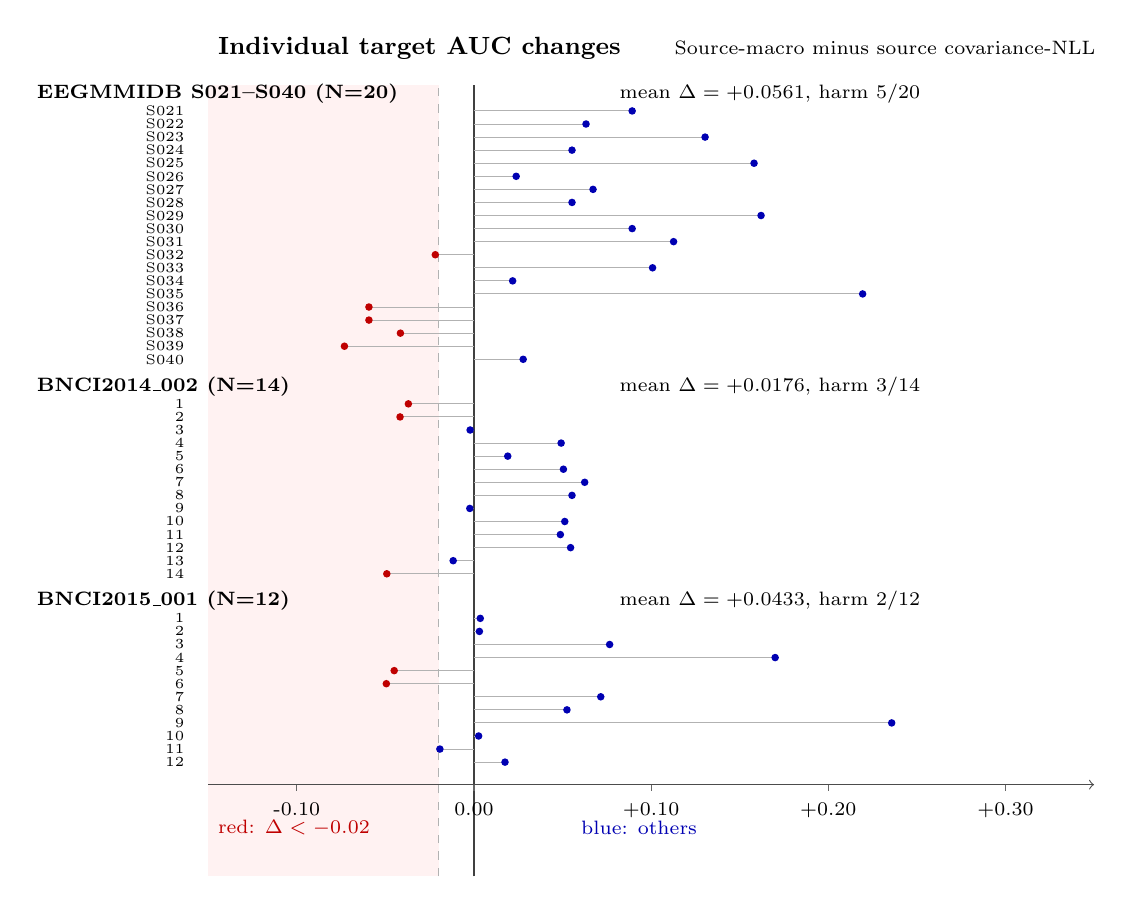
\begin{tikzpicture}[x=1cm,y=1cm]
\fill[red!5] (2.300,1.68) rectangle (5.225,11.73);
\draw[dashed, gray!60] (5.225,1.68) -- (5.225,11.73);
\draw[black!75,line width=0.55pt] (5.675,1.68) -- (5.675,11.73);
\node[anchor=west,font=\small\bfseries] at (2.3,12.2) {Individual target AUC changes};
\node[anchor=west,font=\scriptsize] at (8.1,12.2) {Source-macro minus source covariance-NLL};
\node[anchor=west,font=\scriptsize\bfseries] at (0.0,11.620) {EEGMMIDB S021--S040 (N=20)};
\node[anchor=west,font=\scriptsize] at (7.4,11.620) {mean $\Delta=+0.0561$, harm 5/20};
\node[anchor=east,font=\tiny] at (2.12,11.400) {S021};
\draw[black!30,line width=0.35pt] (5.675,11.400) -- (7.684,11.400);
\fill[blue!70!black] (7.684,11.400) circle (0.048);
\node[anchor=east,font=\tiny] at (2.12,11.234) {S022};
\draw[black!30,line width=0.35pt] (5.675,11.234) -- (7.098,11.234);
\fill[blue!70!black] (7.098,11.234) circle (0.048);
\node[anchor=east,font=\tiny] at (2.12,11.068) {S023};
\draw[black!30,line width=0.35pt] (5.675,11.068) -- (8.610,11.068);
\fill[blue!70!black] (8.610,11.068) circle (0.048);
\node[anchor=east,font=\tiny] at (2.12,10.902) {S024};
\draw[black!30,line width=0.35pt] (5.675,10.902) -- (6.920,10.902);
\fill[blue!70!black] (6.920,10.902) circle (0.048);
\node[anchor=east,font=\tiny] at (2.12,10.736) {S025};
\draw[black!30,line width=0.35pt] (5.675,10.736) -- (9.232,10.736);
\fill[blue!70!black] (9.232,10.736) circle (0.048);
\node[anchor=east,font=\tiny] at (2.12,10.570) {S026};
\draw[black!30,line width=0.35pt] (5.675,10.570) -- (6.211,10.570);
\fill[blue!70!black] (6.211,10.570) circle (0.048);
\node[anchor=east,font=\tiny] at (2.12,10.404) {S027};
\draw[black!30,line width=0.35pt] (5.675,10.404) -- (7.187,10.404);
\fill[blue!70!black] (7.187,10.404) circle (0.048);
\node[anchor=east,font=\tiny] at (2.12,10.238) {S028};
\draw[black!30,line width=0.35pt] (5.675,10.238) -- (6.920,10.238);
\fill[blue!70!black] (6.920,10.238) circle (0.048);
\node[anchor=east,font=\tiny] at (2.12,10.072) {S029};
\draw[black!30,line width=0.35pt] (5.675,10.072) -- (9.321,10.072);
\fill[blue!70!black] (9.321,10.072) circle (0.048);
\node[anchor=east,font=\tiny] at (2.12,9.906) {S030};
\draw[black!30,line width=0.35pt] (5.675,9.906) -- (7.684,9.906);
\fill[blue!70!black] (7.684,9.906) circle (0.048);
\node[anchor=east,font=\tiny] at (2.12,9.740) {S031};
\draw[black!30,line width=0.35pt] (5.675,9.740) -- (8.210,9.740);
\fill[blue!70!black] (8.210,9.740) circle (0.048);
\node[anchor=east,font=\tiny] at (2.12,9.574) {S032};
\draw[black!30,line width=0.35pt] (5.675,9.574) -- (5.184,9.574);
\fill[red!75!black] (5.184,9.574) circle (0.048);
\node[anchor=east,font=\tiny] at (2.12,9.408) {S033};
\draw[black!30,line width=0.35pt] (5.675,9.408) -- (7.943,9.408);
\fill[blue!70!black] (7.943,9.408) circle (0.048);
\node[anchor=east,font=\tiny] at (2.12,9.242) {S034};
\draw[black!30,line width=0.35pt] (5.675,9.242) -- (6.166,9.242);
\fill[blue!70!black] (6.166,9.242) circle (0.048);
\node[anchor=east,font=\tiny] at (2.12,9.076) {S035};
\draw[black!30,line width=0.35pt] (5.675,9.076) -- (10.611,9.076);
\fill[blue!70!black] (10.611,9.076) circle (0.048);
\node[anchor=east,font=\tiny] at (2.12,8.910) {S036};
\draw[black!30,line width=0.35pt] (5.675,8.910) -- (4.341,8.910);
\fill[red!75!black] (4.341,8.910) circle (0.048);
\node[anchor=east,font=\tiny] at (2.12,8.744) {S037};
\draw[black!30,line width=0.35pt] (5.675,8.744) -- (4.341,8.744);
\fill[red!75!black] (4.341,8.744) circle (0.048);
\node[anchor=east,font=\tiny] at (2.12,8.578) {S038};
\draw[black!30,line width=0.35pt] (5.675,8.578) -- (4.741,8.578);
\fill[red!75!black] (4.741,8.578) circle (0.048);
\node[anchor=east,font=\tiny] at (2.12,8.412) {S039};
\draw[black!30,line width=0.35pt] (5.675,8.412) -- (4.030,8.412);
\fill[red!75!black] (4.030,8.412) circle (0.048);
\node[anchor=east,font=\tiny] at (2.12,8.246) {S040};
\draw[black!30,line width=0.35pt] (5.675,8.246) -- (6.300,8.246);
\fill[blue!70!black] (6.300,8.246) circle (0.048);
\node[anchor=west,font=\scriptsize\bfseries] at (0.0,7.900) {BNCI2014\_002 (N=14)};
\node[anchor=west,font=\scriptsize] at (7.4,7.900) {mean $\Delta=+0.0176$, harm 3/14};
\node[anchor=east,font=\tiny] at (2.12,7.680) {1};
\draw[black!30,line width=0.35pt] (5.675,7.680) -- (4.842,7.680);
\fill[red!75!black] (4.842,7.680) circle (0.048);
\node[anchor=east,font=\tiny] at (2.12,7.514) {2};
\draw[black!30,line width=0.35pt] (5.675,7.514) -- (4.736,7.514);
\fill[red!75!black] (4.736,7.514) circle (0.048);
\node[anchor=east,font=\tiny] at (2.12,7.348) {3};
\draw[black!30,line width=0.35pt] (5.675,7.348) -- (5.626,7.348);
\fill[blue!70!black] (5.626,7.348) circle (0.048);
\node[anchor=east,font=\tiny] at (2.12,7.182) {4};
\draw[black!30,line width=0.35pt] (5.675,7.182) -- (6.782,7.182);
\fill[blue!70!black] (6.782,7.182) circle (0.048);
\node[anchor=east,font=\tiny] at (2.12,7.016) {5};
\draw[black!30,line width=0.35pt] (5.675,7.016) -- (6.104,7.016);
\fill[blue!70!black] (6.104,7.016) circle (0.048);
\node[anchor=east,font=\tiny] at (2.12,6.850) {6};
\draw[black!30,line width=0.35pt] (5.675,6.850) -- (6.811,6.850);
\fill[blue!70!black] (6.811,6.850) circle (0.048);
\node[anchor=east,font=\tiny] at (2.12,6.684) {7};
\draw[black!30,line width=0.35pt] (5.675,6.684) -- (7.081,6.684);
\fill[blue!70!black] (7.081,6.684) circle (0.048);
\node[anchor=east,font=\tiny] at (2.12,6.518) {8};
\draw[black!30,line width=0.35pt] (5.675,6.518) -- (6.920,6.518);
\fill[blue!70!black] (6.920,6.518) circle (0.048);
\node[anchor=east,font=\tiny] at (2.12,6.352) {9};
\draw[black!30,line width=0.35pt] (5.675,6.352) -- (5.622,6.352);
\fill[blue!70!black] (5.622,6.352) circle (0.048);
\node[anchor=east,font=\tiny] at (2.12,6.186) {10};
\draw[black!30,line width=0.35pt] (5.675,6.186) -- (6.828,6.186);
\fill[blue!70!black] (6.828,6.186) circle (0.048);
\node[anchor=east,font=\tiny] at (2.12,6.020) {11};
\draw[black!30,line width=0.35pt] (5.675,6.020) -- (6.772,6.020);
\fill[blue!70!black] (6.772,6.020) circle (0.048);
\node[anchor=east,font=\tiny] at (2.12,5.854) {12};
\draw[black!30,line width=0.35pt] (5.675,5.854) -- (6.902,5.854);
\fill[blue!70!black] (6.902,5.854) circle (0.048);
\node[anchor=east,font=\tiny] at (2.12,5.688) {13};
\draw[black!30,line width=0.35pt] (5.675,5.688) -- (5.411,5.688);
\fill[blue!70!black] (5.411,5.688) circle (0.048);
\node[anchor=east,font=\tiny] at (2.12,5.522) {14};
\draw[black!30,line width=0.35pt] (5.675,5.522) -- (4.568,5.522);
\fill[red!75!black] (4.568,5.522) circle (0.048);
\node[anchor=west,font=\scriptsize\bfseries] at (0.0,5.176) {BNCI2015\_001 (N=12)};
\node[anchor=west,font=\scriptsize] at (7.4,5.176) {mean $\Delta=+0.0433$, harm 2/12};
\node[anchor=east,font=\tiny] at (2.12,4.956) {1};
\draw[black!30,line width=0.35pt] (5.675,4.956) -- (5.755,4.956);
\fill[blue!70!black] (5.755,4.956) circle (0.048);
\node[anchor=east,font=\tiny] at (2.12,4.790) {2};
\draw[black!30,line width=0.35pt] (5.675,4.790) -- (5.744,4.790);
\fill[blue!70!black] (5.744,4.790) circle (0.048);
\node[anchor=east,font=\tiny] at (2.12,4.624) {3};
\draw[black!30,line width=0.35pt] (5.675,4.624) -- (7.398,4.624);
\fill[blue!70!black] (7.398,4.624) circle (0.048);
\node[anchor=east,font=\tiny] at (2.12,4.458) {4};
\draw[black!30,line width=0.35pt] (5.675,4.458) -- (9.500,4.458);
\fill[blue!70!black] (9.500,4.458) circle (0.048);
\node[anchor=east,font=\tiny] at (2.12,4.292) {5};
\draw[black!30,line width=0.35pt] (5.675,4.292) -- (4.662,4.292);
\fill[red!75!black] (4.662,4.292) circle (0.048);
\node[anchor=east,font=\tiny] at (2.12,4.126) {6};
\draw[black!30,line width=0.35pt] (5.675,4.126) -- (4.562,4.126);
\fill[red!75!black] (4.562,4.126) circle (0.048);
\node[anchor=east,font=\tiny] at (2.12,3.960) {7};
\draw[black!30,line width=0.35pt] (5.675,3.960) -- (7.285,3.960);
\fill[blue!70!black] (7.285,3.960) circle (0.048);
\node[anchor=east,font=\tiny] at (2.12,3.794) {8};
\draw[black!30,line width=0.35pt] (5.675,3.794) -- (6.856,3.794);
\fill[blue!70!black] (6.856,3.794) circle (0.048);
\node[anchor=east,font=\tiny] at (2.12,3.628) {9};
\draw[black!30,line width=0.35pt] (5.675,3.628) -- (10.980,3.628);
\fill[blue!70!black] (10.980,3.628) circle (0.048);
\node[anchor=east,font=\tiny] at (2.12,3.462) {10};
\draw[black!30,line width=0.35pt] (5.675,3.462) -- (5.734,3.462);
\fill[blue!70!black] (5.734,3.462) circle (0.048);
\node[anchor=east,font=\tiny] at (2.12,3.296) {11};
\draw[black!30,line width=0.35pt] (5.675,3.296) -- (5.242,3.296);
\fill[blue!70!black] (5.242,3.296) circle (0.048);
\node[anchor=east,font=\tiny] at (2.12,3.130) {12};
\draw[black!30,line width=0.35pt] (5.675,3.130) -- (6.069,3.130);
\fill[blue!70!black] (6.069,3.130) circle (0.048);
\draw[->,black!70] (2.300,2.844) -- (13.550,2.844);
\draw[black!60] (3.425,2.844) -- (3.425,2.764);
\node[anchor=north,font=\scriptsize] at (3.425,2.734) {-0.10};
\draw[black!60] (5.675,2.844) -- (5.675,2.764);
\node[anchor=north,font=\scriptsize] at (5.675,2.734) {0.00};
\draw[black!60] (7.925,2.844) -- (7.925,2.764);
\node[anchor=north,font=\scriptsize] at (7.925,2.734) {+0.10};
\draw[black!60] (10.175,2.844) -- (10.175,2.764);
\node[anchor=north,font=\scriptsize] at (10.175,2.734) {+0.20};
\draw[black!60] (12.425,2.844) -- (12.425,2.764);
\node[anchor=north,font=\scriptsize] at (12.425,2.734) {+0.30};
\node[anchor=west,font=\scriptsize,red!75!black] at (2.300,2.294) {red: $\Delta<-0.02$};
\node[anchor=west,font=\scriptsize,blue!70!black] at (6.912,2.294) {blue: others};
\end{tikzpicture}
\caption{Paired participant-level target AUC differences between the frozen source participant-macro selector and the source covariance-NLL selector in three EEG cohorts. Five of 20, three of 14 and two of 12 participants, respectively, lost more than 0.02 AUC. The vertical reference line is zero, and the tinted region denotes the material-harm threshold. EEGMMIDB was a prospectively frozen within-database block; both BNCI datasets were TRUE PRE-DATA external cohorts whose Holm-adjusted primary comparisons remain individually inconclusive. Points are descriptive and must not be treated as independent trials or a new confirmatory family.}
\label{fig:participant-harm-v10}
\end{figure*}

# SNAPSHOT_SOURCE: lindicaphxag-tech/cs@0b26a5b0853e3b136a92c17e614a3a1936673621 path=papers/eeg-default-regularisation/paper_vnext/03_discussion_current.tex
\section{Discussion}

The reconstruction supports a different paper from the one suggested by the
historical draft. The strongest result is not a new shrinkage estimator and
not a universal multiplier. It is a validity result: covariance fidelity and
cross-participant discrimination can define different regularisation regimes,
and the choice between those objectives can alter both held-participant
performance and the scientific conclusion drawn from an EEG representation
comparison.

The operator analysis clarifies why this is possible without claiming that
the abstract distinction between covariance estimation and classification is
new. Along the scalar shrinkage path, the standardized evaluation margin is
invariant to the component of \(w_\lambda'\) that merely rescales the
discriminant. Only the component that rotates the discriminant in the
evaluation participant's covariance geometry can change the margin. The
covariance-predictive derivative, by contrast, contains no class-contrast
vector. Hence covariance stationarity provides no general guarantee of
discriminative stationarity. Near an interior covariance optimum, the
covariance loss can be locally flat to first order while the discriminative
margin changes to first order. This local asymptotic statement is conditional:
it does not apply unchanged when the covariance optimum lies on the boundary
of the admissible path. That distinction is empirically relevant here,
because BNCI2014\_002 selects \(\lambda_C=0\) in 13/14 outer folds,
whereas BNCI2015\_001 selects interior values between 0.015 and 0.05. The
Validity Frontier is therefore the primary empirical object in both cohorts;
the local square-root mechanism is a compatible explanation only where its
interior-optimum assumptions hold. The frontier measures how much decision
variation is admitted by a given fidelity tolerance rather than treating
numerical proximity in covariance loss as evidence of decision equivalence.

The EEGMMIDB S021--S040 block establishes that this distinction can have a
large prospective consequence. Source participant-discrimination selection
improved macro AUC by approximately 0.056 over the stronger source
covariance-NLL criterion and by 0.092 over Ledoit--Wolf, with both predeclared
comparisons surviving Holm correction. The delete-one-source reselection
audit is important because it changes the object that appears stable. The
selected numerical strength moves from 0.4 to 0.95 when source composition is
perturbed, whereas the ordering of source objectives retains a positive target
consequence in all eight omissions. The empirical regularity is therefore not
that \(\lambda=0.8\) is the correct EEG value; it is that a
discrimination-matched source objective can occupy a different region from a
covariance-matched objective and can transfer better under this protocol.

The TRUE PRE-DATA external panel strengthens and simultaneously narrows that
claim. BNCI2014\_002 and BNCI2015\_001 differ in acquisition geometry,
channel count, tangent dimension, trial count and session structure, yet the
two source objectives select different regularisation regions in 26/26 outer
folds. The target-effect direction is also positive in both datasets:
source-macro selection exceeds covariance-NLL by +0.0176 and +0.0433 AUC,
respectively, and exceeds Ledoit--Wolf by +0.0229 and +0.0453. However,
neither external dataset passes its own frozen exact sign-flip plus Holm
family. We therefore regard the source-objective separation as strongly
replicated in the studied motor-imagery cohorts and the target-performance
consequence as directionally replicated, not as two additional individually
significant superiority experiments. The distinction matters because the
participant bootstrap intervals and exact randomisation tests answer related
but non-identical finite-sample questions; choosing whichever is more
favourable after seeing the outcome would defeat the purpose of the pre-data
protocol.

The corrected Validity Frontier adds a second form of external replication.
The observed max-minus-min AUC spans exceed 0.02 over the frozen dense
regularisation path in both TRUE PRE-DATA cohorts. Yet a positive percentile
bootstrap lower endpoint for a data-selected maximum span does not by itself
establish a population-level material path effect: even a flat population AUC
path can produce a positive empirical max--min span from sampling noise across
hundreds of lambda points. We therefore report these frontiers as descriptive
post-score measurements and add an explicitly post-outcome simultaneous-path
sensitivity diagnostic, rather than interpreting the original percentile
intervals as proof of materiality. The raw fidelity budget required to
reach a 0.02 span differs substantially: approximately 0.916 per-dimension
NLL-regret units in BNCI2014\_002 and 0.175 in BNCI2015\_001. This
heterogeneity is scientifically useful. It rejects the idea of one universal
critical fidelity tolerance while supporting a more general statement that
covariance fidelity defines a cohort-dependent decision-validity frontier.
The dense-grid subset audit further shows that the observed spans are not an
artifact of one particular grid resolution.

The prospective representation experiment demonstrates why this validity
question matters beyond classifier tuning. The regularisation objective
significantly changes the filter-bank-versus-wideband contrast, but the
direction is the opposite of the historical hypothesis:
discrimination-oriented regularisation strengthens the wide-band advantage
rather than uncovering a hidden filter-bank gain. The matched-dimension PCA
control remains below WIDE231, while the nuisance-dimension and source-budget
interventions do not support a simple monotonic feature-to-sample explanation.
Thus the paper does not rescue its original representation story. It
prospectively falsifies it while preserving the more general conclusion that
regularisation objective can alter representation-level inference. This is a
stronger measurement-validity result than a post-hoc ranking reversal selected
because it supports the original narrative.

The failed algorithmic corrections are similarly informative. Lower-tail
signed selection did not beat correctly nested source tuning; CFCTS was
prospectively inferior; FCTR collapses toward a covariance-fidelity region
that underperformed on S021--S040; the TRUE PRE-DATA mean--tail--fidelity
selector does not satisfy its frozen two-cohort tail promotion gate; and the
post-S021 discriminability-first lexicographic rule is slightly worse than
pure source-macro selection in both external cohorts. These results eliminate
several plausible but unsupported claims of algorithmic novelty. They also
suggest that the difficult part of the problem is not constructing a more
ornate scalar selector. Participant heterogeneity creates a trade-off between
mean transfer benefit and harmed-participant risk that is not resolved by a
single source-only tie-breaker in the present data.

The S061--S080 calibration-budget experiment provides another useful
negative result. Its unlabeled adaptation subtracts one constant
participant-specific feature translation before a fixed linear score.
Because this only adds a constant to every score from that participant,
within-participant ROC ordering cannot change and ROC AUC is algebraically
invariant. The observed zero U-\(k\)/Z0 AUC differences are therefore not
evidence that unlabeled calibration is practically useless. They expose an
endpoint--operator identifiability mismatch. A future practical BCI extension
must use a source-frozen operating threshold or another threshold-sensitive
utility measure; such an extension is necessarily later than the current
outcome and cannot be presented as part of the original prospective claim.

These findings also define the novelty boundary relative to prior work.
Covariance shrinkage, regularised discriminant analysis, participant-wise
cross-validation, Riemannian tangent features and zero-calibration transfer
are established techniques, and recent EEG work has explicitly studied the
effects of regularisation and validation choices. The contribution here is
therefore not the observation that a hyperparameter influences accuracy. It
is the combined, auditable chain from objective-specific operator geometry to
full-domain source conflict, prospective target consequence, source-pool
sensitivity, true-pre-data external replication, uncertainty-aware validity
frontiers and prospective falsification of a representation conclusion under
one information budget.

Several limits remain. The strongest external evidence is currently confined
to motor imagery, and all headline regularisation results use linear
discriminants on covariance/tangent representations. The two TRUE PRE-DATA
external cohorts are independent acquisition strata but still too few for a
general EEG-wide law or a meaningful dataset-level meta-analysis. AUC measures
ranking and does not by itself establish calibrated operating-point utility.
The harmed-participant tail remains non-trivial even when the average effect
is favourable. Finally, the operator derivation identifies a local mechanism
but has not yet been promoted to a target-label-free predictor of who will
benefit; doing so would require a new independently frozen experiment rather
than reusing the current target outcomes.

For these reasons, the present scope is deliberately narrower than the
historical title implied. The evidence supports a BSPC-style
signal-processing and measurement-validity contribution in the studied
cross-subject covariance/tangent discriminant family. A JNE submission becomes
plausible if the final paper emphasizes the neural-engineering consequence of
representation-dependent validity and preserves the unusually strict evidence
chain. TNSRE would still require a separate direct BCI-utility extension,
preferably threshold-sensitive, cross-session/device or online-like. Stronger
wording cannot substitute for that evidence.

\section{Conclusions}
In the studied zero-target covariance/tangent-space discriminant pipelines,
source covariance fidelity and source held-participant discrimination favor
different finite-grid shrinkage regimes. A prospectively frozen EEGMMIDB block
shows that the choice has a real held-participant AUC consequence; two
independently frozen external datasets preserve the effect direction but do
not individually establish Holm-adjusted superiority. A second prospective
experiment shows that the same choice can change a spectral-representation
comparison, while refuting the historical filter-bank advantage. The
regularisation validity frontier remains descriptive pending simultaneous
path-level and source-pool uncertainty checks. These results warrant
treating the regularisation objective as an explicit EEG measurement choice,
not assuming that a covariance-estimation optimum is a transferable
discrimination optimum or a universally superior selector.
\clearpage
\begin{table*}[t]
\centering
\caption{Prospective and TRUE PRE-DATA Z0 evidence for regularisation-objective mismatch. AUC values are participant-macro averages. $\Delta_{\mathrm{cov}}$ compares full-domain source participant-discrimination selection with source covariance-NLL selection; $\Delta_{\mathrm{LW}}$ compares it with analytic Ledoit--Wolf. Confidence intervals are participant bootstrap intervals. Holm $p$ values belong to the frozen two-comparison family within each cohort. External cohorts are replication strata and are not pooled for significance.}
\label{tab:main-prospective-results}
\scriptsize
\setlength{\tabcolsep}{3.2pt}
\renewcommand{\arraystretch}{1.12}
\begin{tabular}{lrrrrcrcr}
\toprule
Cohort & $N$ & Macro & Cov-NLL & LW &
\shortstack{$\Delta_{\mathrm{cov}}$\\95\% CI} &
Holm $p$ &
\shortstack{$\Delta_{\mathrm{LW}}$\\95\% CI} &
Holm $p$ \\
\midrule
EEGMMIDB S021--S040
& 20 & 0.7212 & 0.6651 & 0.6292
& \shortstack{+0.0561\\[0.0218, 0.0905]}
& 0.0060
& \shortstack{+0.0920\\[0.0411, 0.1431]}
& 0.0051 \\
BNCI2014\_002
& 14 & 0.7781 & 0.7605 & 0.7552
& \shortstack{+0.0176\\[-0.0036, 0.0373]}
& 0.1396
& \shortstack{+0.0229\\[0.0004, 0.0440]}
& 0.1396 \\
BNCI2015\_001
& 12 & 0.7670 & 0.7237 & 0.7217
& \shortstack{+0.0433\\[0.0002, 0.0935]}
& 0.1855
& \shortstack{+0.0453\\[0.0029, 0.0957]}
& 0.1855 \\
\bottomrule
\end{tabular}

\vspace{1mm}
\footnotesize
S021--S040 is a prospectively frozen within-database confirmation; BNCI2014\_002 and BNCI2015\_001 are independently recorded TRUE PRE-DATA external cohorts under one unchanged v5 protocol. The external target-effect direction is positive in both datasets, but neither external exact sign-flip + Holm family is individually significant. Harmed-participant tails are reported separately and are not hidden by the macro averages.
\end{table*}

# SNAPSHOT_SOURCE: lindicaphxag-tech/cs@0b26a5b0853e3b136a92c17e614a3a1936673621 path=papers/eeg-default-regularisation/paper_vnext/92_table_validity_frontier.tex
\begin{table}[t]
\centering
\caption{Corrected TRUE PRE-DATA Regularisation Validity Frontiers. The primary material-fragility threshold is a 0.02 AUC envelope span. $\delta_{0.02}$ is expressed in raw per-dimension source covariance predictive-NLL regret. Percentile intervals describe 20,000 paired participant-path resamples; they are not simultaneous confidence bands or tests of a data-selected positive range.}
\label{tab:validity-frontier}
\small
\begin{tabular}{lrrr}
\hline
Cohort & Max AUC span (95\% CI) & $\delta_{0.02}$ & Finite bootstrap fraction \\
\hline
BNCI2014\_002
& 0.0384 [0.0271, 0.0666]
& 0.9161
& 0.9995 \\
BNCI2015\_001
& 0.0501 [0.0224, 0.1034]
& 0.1752
& 0.9877 \\
\hline
\end{tabular}

\vspace{1mm}
\footnotesize
Both cohorts admit a material downstream AUC span over the frozen dense regularisation path, but the critical raw fidelity budget differs substantially. The supported conclusion is therefore a reproducible, cohort-dependent validity frontier rather than one universal critical $\delta$. The obsolete generic centered-AUC zero-crossing statistic is not used.
\end{table}

\bibliographystyle{unsrt}
\bibliography{references_v10}
\end{document}
